\begin{figure*}[htbp]
    \centering
    
    % --- STOLPEC (a) ---
    \begin{subfigure}[b]{0.3\textwidth}
        \centering
        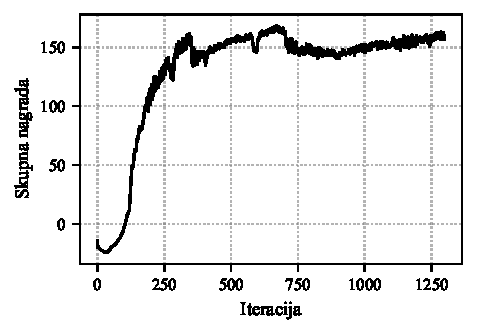
\includegraphics[width=\textwidth]{Images/Episode_reward.pdf}
        \caption{}
        \label{Nagrada}
    \end{subfigure}
    \hfill % Avtomatski vodoravni razmak med stolpci
  % --- STOLPEC (b) ---
    \begin{subfigure}[b]{0.3\textwidth}
        \centering
        \includegraphics[width=\textwidth]{Images/Mean_episode_length.pdf}
        \caption{}
        \label{Dolžina epizode}
    \end{subfigure}
    \hfill % Avtomatski vodoravni razmak med stolpci
  % --- STOLPEC (d) ---
    \begin{subfigure}[b]{0.3\textwidth}
        \centering
        \includegraphics[width=\textwidth]{Images/Position_penalty.pdf}
        \caption{}
        \label{Kazen pozicije}
    \end{subfigure}
    \hfill % Avtomatski vodoravni razmak med stolpci
    % --- STOLPEC (c) ---
    \begin{subfigure}[b]{0.3\textwidth}
        \centering
        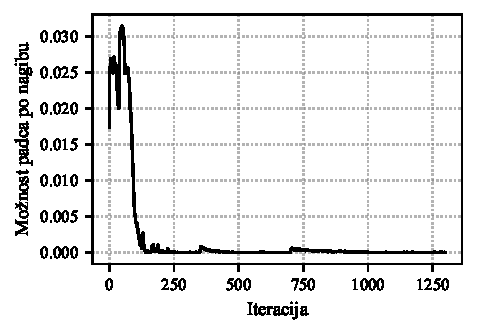
\includegraphics[width=\textwidth]{Images/Roll_fall_rate.pdf}
        \caption{}
        \label{Padec nagiba}
    \end{subfigure}
    \hfill % Avtomatski vodoravni razmak med stolpci
      % --- STOLPEC (c) ---
    \begin{subfigure}[b]{0.3\textwidth}
        \centering
        \includegraphics[width=\textwidth]{Images/roll_rate_penalty.pdf}
        \caption{}
        \label{Hitrost nagiba}
    \end{subfigure}
    \hfill % Avtomatski vodoravni razmak med stolpci
    % --- STOLPEC (c) ---
    \begin{subfigure}[b]{0.3\textwidth}
        \centering
        \includegraphics[width=\textwidth]{Images/pitch_rate_penalty.pdf}
        \caption{}
        \label{Hitrost naklona}
    \end{subfigure}
    \hfill % Avtomatski vodoravni razmak med stolpci

    \caption{(a) Položaj ter diferencial kotov med manevriranjem, (b) Sprememba želenega kota $\varphi$ za ohranjanje položaja, (c) Stanje $\varphi$ med postavitvijo robota iz ležečega položaja.}
    \label{fig:glavna_slika_6}
\end{figure*} 

\section{Eksperimentalni rezultati}
  V grafu pridobljene nagrade na epizodo \ref{Nagrada} se lepo vidijo preskoki različnih faz večfaznega učenja. Na začetku se opazi, da nagrada konvergira navzgor, strmo pade pri prestopu v drugo fazo po 500 iteracijah, nadaljuje s strmo rastjo in se ustali nekje na vrednosti 120, nakar strmo pade ob začetku tretje faze po 800 iteracijah. Nagrada nato postopoma raste in ne doživi več tako strmih padcev kljub prestopu v četrto fazo v iteraciji 1100. Ti preskoki med fazami, so še lažje opazni na grafu \ref{Padec nagiba}, kjer se ob vsaki spremembi faze vidi vedno večjo naklonjenost padcu preko nagiba robota. Opazimo lahko, da se stabilizacija ne izboljšuje z enako mero v 3. in 4. fazi, kot se v 1. in 2.. Na to tudi kaže graf \ref{Dolžina epizode}, Kateri nakazuje na to da po prehodu v 3. fazo čas epizode drastično pade in se povečuje počasneje napram prvima dvema fazama.
Kazen po poziciji nakazuje na stabilen sistem, na katerem se večfazno učenje ne da opaziti zlahko. Opazimo lahko, da absolutna vrednost kazni strmo pade in do konca učnega cikla ohrani nekoliko enakomerno vrednost brez velikih spremeb. 
  Ker robot lovi ravnotežje s pomočjo motorjev M1, M2 in M3 se neprestano pomika naprej nazaj ter gor in dol, zaradi česar na grafih \ref{Hitrost nagiba} in \ref{Hitrost naklona} vidimo konvergiranje azni proti določeni vrednosti, kjer se kazen ustali. To je prilakovano že zaradi strukture samega problema.
  
  